
%*********************************************************************%
%                                                                     %
%              Introduction section                                   %
%                                                                     %
%*********************************************************************%


\chapter{Convection, Rotation and Magnetism}
\label{chapter:introduction}

We live near a magnetic star and our Earth is embedded within its
magnetized wind.  The surface of the Sun is covered in magnetism on all
scales, with global-scale structures including prominences that reach
high into the solar atmosphere (Fig.~\ref{fig:solar magnetism}$a$) as
well as smaller concentrated magnetic structures like sunspots, where
the magnetism becomes strong enough to largely halt the turbulent
convection leaving dark regions at the surface (Fig.~\ref{fig:solar
  magnetism}$b$).  On the smallest scales visible at the surface,
magnetic fields are swept aside by vigorous granulation which
are convective cells that overturn every 10-15 minutes and have flows
that are near the speed of sound.  The magnetism collects in
the surrounding network of downflow lanes, where it is swept out by
the slower flows of supergranulation, whose characteristic timescales
are closer to a day.  There the magnetism traces out the supergranular
network, and expands outwards into the solar chromosphere and corona.

Solar magnetism is far from being static, and it evolves on many timescales, with a
prominent and regular eleven-year cycle of sunspots and global-scale
polarity reversals. We stand at the start of a new cycle now (called cycle~24); few
sunspots are present on the solar disk and eruptive events and space
storms are rare.  Over the next eleven years we will likely see spots
emerging at the surface, initially at higher latitudes (near
$\pm30^\circ$) and then at lower and lower latitudes until, near the
end of the cycle, they appear almost at the solar
equator. Time-latitude maps of spot emergence form characteristic
``butterfly'' patterns and these diagrams illustrate the migration of
the active latitudes as the cycle progresses (Fig.\ref{fig:butterfly
  diagram}$a$). When sunspots emerge at the solar surface, they
generally have characteristic polarities and orientations.  Spots can
be large or small, with most as large as the Earth or larger.   


\begin{figure}[!t]
  \begin{center}
    \includegraphics[width=0.8\linewidth]{figs/chapter_1/solar_magnetism_examples.eps}
  \end{center}
  \caption[Solar magnetism at many scales]{Solar magnetism at many
    scales.  $(a)$~On global-scales, a large
    prominence lifting off the limb of the Sun is 
    revealed in this SOHO EIT image.  A scaled-image of the Earth
    (inside blue circle) is provided for comparison. 
    $(b)$~On~finer scales, as seen in this image from the SSVT,
    sunspots at the surface are regions of
    strong magnetism.  Tick marks indicate 1Mm spacings.  Individual
    sunspots are roughly the size of the Earth.
    \label{fig:solar magnetism}}
\end{figure}

Within the sunspots, the magnetism can evolve on very short
timescales.  In some active regions the strong magnetic fields reconnect, leading to
explosive releases of energy in the form of high-energy photon flares 
and eruptive plasma coronal mass ejections.  As these photons and
magnetized plasma storms strike the Earth's magnetosphere, they can
profoundly affect our modern society, imperiling astronauts and
satellites in space and scrambling communications and navigation
systems on the ground.  The largest solar storms can threaten the 
very infrastructure of national power grids and can disrupt or
destroy computational systems.   

As the cycle progresses, the sunspots will become more numerous, peaking in
number roughly midway through (Fig.~\ref{fig:butterfly diagram}$b$).
Generally, the number of sunspots present on the solar disk increases
rapidly at the start of a new solar cycle and then declines more gradually.
It is during the later half of the 
cycle that the largest storms and eruptive events tend to occur,
though major flares and eruptions can occur at any time.  
Near the middle of the roughly eleven-year solar cycle, when the
number of sunspots is near maximum, the magnetic poles of the Sun flip in polarity.  As the number of sunspots
declines and the active latitudes approach the equator, a cycle begins
anew with sunspots of opposite polarity emerging at high latitudes.   
Though the timing of the solar cycle is fairly regular, the
magnetic activity shows modulation on longer timescales as well. Some
cycles are strong, with many spots, while some cycles are weak. At
times,as during the Maunder Minimum, the surface of the Sun has
remained barren of sunspots for decades. 


\begin{figure}[!t]
  \begin{center}
    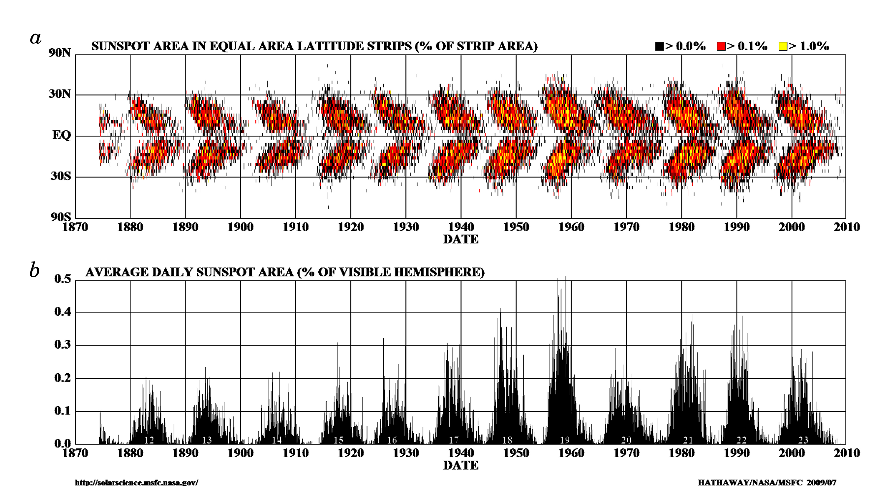
\includegraphics[width=\linewidth]{figs/chapter_1/Hathaway_butterfly_diagram_073009.eps}
  \end{center}
  \caption[Temporal variation of global-scale solar magnetism]
          {Temporal variation of global-scale solar magnetism.
            $(a)$~Butterfly diagram, or time-latitude map, showing
            emergence of sunspots at the surface.  When a new cycle
            begins, sunspots emerge first at high latitudes.  As time
            passes, they become more numerous and appear at lower
            latitudes.  When their number is near maximum, the global-scale
            polarities reverse.  As their number declines and the
            sunspots approach the equator, a cycle begins anew with
            opposite polarity sunspots.
            $(b)$~Percentage of the visible solar disk that is
            covered by sunspots.  These figures adapted from
            \cite{Hathaway_2009}. 
            \label{fig:butterfly diagram}}
          \vskip-0.5cm
\end{figure}



\section{Operation of the Solar Dynamo}
Solar magnetism and the cycles of magnetic activity must arise from
organized dynamo action in the Sun's interior.  This dynamo
action is achieved by turbulent plasma motions
in the solar convection zone, which spans the outer 29\%
of the Sun in radius.  Here vigorous convective motions and rotation
couple to drive the differential rotation and
meridional circulation.  These flows are important ingredients in
stellar dynamo theory, and in many theories the differential rotation
plays an  important role in building and organizing the global-scale
fields. The meridional circulations may be important for returning flux
to the base of the convection zone and advecting it equatorward,
enabling cycles of magnetic activity.  

The manner in which the Sun achieves global-scale dynamo action is
gradually being sorted out.  
The seat of this dynamo is generally thought to
be located in the tachocline, an interface of shear between the
differentially rotating convection zone and the radiative interior
which is in solid body rotation
\citep[e.g.,][]{Parker_1993,Charbonneau&MacGregor_1997,Ossendrijver_2003}. 
Helioseismology, which uses acoustic
oscillations to probe the radial structure of the Sun as well as
convective flows beneath the surface, has revealed that the solar
differential rotation profile observed at the surface prints
throughout the bulk of the convection zone with two important regions
of shear (Fig.~\ref{fig:solar DR and Brummell diagram}$a$).  
The near-surface shear layer occupies the outer 5\%
of the Sun while the tachocline is at the base of the convection zone
and separates the strong differential rotation of that region from the
uniform rotation of the deeper radiative interior
\citep[e.g.,][]{Thompson_et_al_2003, Thompson_2009}.


The stably stratified
tachocline may also provide a region for storing and amplifying
coherent tubes of magnetic field which may eventually rise to the
surface of the Sun as sunspots.  It has generally been believed that
magnetic buoyancy instabilities may prevent fields from being strongly
amplified within the bulk of the convection zone itself
\citep{Parker_1975}.  In the now prevalent ``interface dynamo'' model,
solar magnetic fields are partly generated in the convection zone by
helical convection, then transported downward into the tachocline
where they are organized and amplified by the shear.  Ultimately the
fields may become unstable and rise to the surface.  This model is
illustrated in Figure~\ref{fig:solar DR and Brummell diagram}$b$.

\begin{figure}[!t]
  \begin{center}
    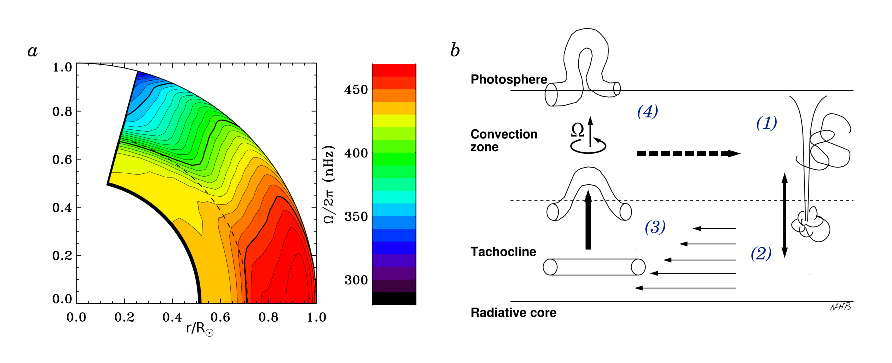
\includegraphics{figs/chapter_1/solar_DR_and_nics_sketch.eps}
  \end{center}
  \caption[Differential rotation and the solar dynamo]
	  {Differential rotation and the solar dynamo.  
     $(a)$~Helioseismically determined differential rotation profile
	  for the Sun, showing the best determination to date of the
	  internal angular velocity $\Omega$ profile \citep{Thompson_2009},
	  with fast (red) equator and slow (blue) poles.
	  Two layers of radial shear are prominently
	  visible, one near the surface and one at the interface
	  between the convection zone and the radiative interior.
	  This deeper layer, the tachocline, may be the seat
	  of the global solar dynamo.
     $(b)$~Sketch of processes likely at work in the solar dynamo.
	  In interface dynamo models, magnetic fields in the convection zone
	  are wound up by helical convective flows~(1) and pumped downwards
	  into the tachocline by the compressible convection~(2).
	  There the field is organized and stretched into global-scale
	  structures~(3) which may become buoyantly unstable
	  and rise to emerge at the surface as sunspots~(4).  As they
	  transit the convection zone, the magnetic tubes are
	  influenced by rotation and some of the field is shredded by
	  convection, closing the loop back to (1).  Meridional
	  circulations may additionally contribute to the transport of
	  field down to the tachocline.
          \label{fig:solar DR and Brummell diagram}}
          \vskip-0.5cm
\end{figure}

In the interface dynamo model, magnetic fields are amplified by
turbulent flows throughout the convection zone.  This ``magnetic
chaff'' is pumped downwards into the tachocline by asymmetries in the
compressible convection, which generally has fast and narrow downflows
and slower and broader upflows.  In the tachocline, the fluctuating
magnetic fields are stored and gradually stretched out by the
differential rotation into
global-scale coherent sheets of magnetism.  These magnetic sheets
become strong enough to undergo magnetic buoyancy instabilities, and
this may break up the sheet into rising magnetic tubes of
predominantly toroidal magnetic field.  If these
tubes survive their transit of the convection zone, they emerge at the
surface as sunspots.  Coriolis forces cause the rising tubes to twist,
which leads to the observed tilt angle of emerging sunspots and may
contribute to the global-scale poloidal field.  

Though some tubes of magnetism may survive, many more are likely to be shredded by
the intense turbulence in the convection zone.  Generally, to emerge
at the surface, the average magnetic energy density of the tube must exceed
the kinetic energy density of the strongest downflows that the tube encounters
during its rise \citep[e.g.,][]{Cline_thesis,Fan_et_al_2003,Abbett_et_al_2004,Jouve&Brun_2009}.  
This strong criteria may be difficult to satisfy in the solar tachocline
\citep{Vasil&Brummell_2008,Vasil&Brummell_2009}.
As the magnetic structures are shredded, helical
convection twists the toroidal field into poloidal field. 
This poloidal field is amplified in the convection zone before being
caught in the vigorous downflows and pumped into the tachocline
closing the loop on the dynamo circuit, though some may also be
transported by the global-scale meridional circulations.  This dynamo
model and the cartoon sketch shown in Figure~\ref{fig:solar DR and Brummell diagram}$b$
summarize the fundamental features found in most modern solar dynamo
theories \citep[e.g.,][]{Charbonneau_2005, Miesch_2005}.


\section{Theoretical Treatments of Stellar Convection}
The elements of the solar dynamo are often interpreted in a mean-field
framework, where the complex turbulent correlations in the induction
equation are linearized in terms of the global-scale magnetic fields.
In these approaches, the magnetism and plasma flows of the interior
are separated into mean components and fluctuations about those
means.  These means are usually taken over large spatial scales and long
temporal epochs, and are often assumed to be much larger in amplitude
than the fluctuating magnetic and velocity fields.

The language of mean-field theory has become the language of dynamo
theory.  In this terminology, the production of mean poloidal field
through the winding up of toroidal field by helical convection is
called an $\alpha$-effect \citep[e.g.,][]{Moffatt_1978, Steenbeck_et_al_1966}. 
The stretching of mean poloidal field into mean toroidal field by the
shearing flows of differential rotation is called an $\Omega$-effect.


In the solar dynamo, the tachocline of shear at the base of the
convection zone is thought to play a key role by providing a region
where the $\Omega$-effect can operate without turbulent convection
shredding and disrupting the global-scale toroidal fields.  The fields
there are thought to grow in strength until magnetic buoyancy carries
them upwards into the convection zone.  There, some of this toroidal
field is shredded and turned into poloidal field by the
$\alpha$-effect from the convection and by Coriolis forces on the
rising tube.  Some flux survives to erupt at the solar surface, creating
sunspots, active regions and, eventually, explosive solar magnetic
activity.  Some of the poloidal field generated by this process is pumped
downward by convection into the tachocline where it is amplified into
toroidal field, thus completing the dynamo cycle.  Conceptual models
similar to this are called ``$\alpha-\Omega$'' dynamos, with the
$\alpha$-effect dominating the production of poloidal field and the
$\Omega$-effect largely responsible for the production of the toroidal
fields.  These models and variants incorporating the global-scale
flow of meridional circulations have shaped our current views on
solar and stellar magnetism.  
Other variants including $\alpha^2$ and 
$\alpha^2\Omega$ dynamos are also proposed for the Sun and
particularly for other stars
\citep[e.g.,][]{Kuker&Rudiger_1999,Kuker&Rudiger_2005_AN, Chabrier&Kuker_2006}.   


Though instructive, these theories
fall short in describing the fully nonlinear dynamo processes occurring
in real stars.  A fundamental assumption of mean-field theories is that the
large-scale fields can be separated from the small-scale fluctuations,
and in these theories the fluctuations are often assumed to scale in
strength with the mean fields.  In the turbulent environment of
stellar convection, fields of all scales interact and are of similar
magnitude, with strong local fluctuations that are not dependent on
the weaker large-scale fields.  Major 3-D simulations
\citep[e.g.,][]{Brun_et_al_2004, Browning_et_al_2006}
and observations suggest that,
at least in the bulk of the convection zone, magnetism occurs over a
broad range of scales with little separation between ``mean'' scales
and fluctuations, and that the mean fields are not the dominant
players in the overall magnetism.  The impact of this lack of scale
separation in both the magnetic and velocity fields is unclear and a
subject of active research in both the dynamo and turbulence
communities.  As an additional concern, mean-field theory is
fundamentally a linear theory, and while it can describe the initial
growth of magnetic fields it cannot address their ultimate saturation
as the fields strengthen and react back on the flows that create
them.  Some attempts have been made to include such nonlinear
effects, with ``$\alpha$-quenching'' and ``$\Omega$-quenching'' terms
added to the mean-field equations, but such treatments are fairly
ad-hoc and the subject of substantial debate.


\section{Exploring Magnetism in Other Stars} 
Our Sun is not the only magnetic star.  Indeed, magnetism appears to be a
ubiquitous feature in stars across the Hertzsprung-Russell (H-R) diagram.  
When our Sun was younger, it must have rotated much more
rapidly, as is suggested both by the solar wind which continually removes
angular momentum from the Sun and by many observations of rapidly
rotating solar-like stars.  Some of these young suns are observed to
rotate as much as 50 times faster than the current solar rate.  
In more rapidly rotating suns the
coupling between rotation and convection is strong and must continue to drive 
global scales of flow.  These young solar-type stars, which rotate
much more rapidly than the sun's current rate, possess much stronger
magnetic activity.   


Rotation appears to be inextricably linked to stellar magnetic activity.
Observations indicate that in stars with extensive convective envelopes,
chromospheric and coronal activity -- which partly trace magnetic heating
of stellar atmospheres -- first rise with increasing rotation rate, then
eventually level off at a constant value for rotation rates above a
mass-dependent threshold velocity \citep[e.g.,][]{Noyes_et_al_1984a, 
Patten&Simon_1996, Delfosse_et_al_1998, Pizzolato_et_al_2003}. Activity may even decline somewhat in the
most rapid rotators \citep[e.g.,][]{James_et_al_2000}.  
This rotation-activity correlation is shown in
Figure~\ref{fig:observations of stars}$a,b$ for a variety of solar-like
stars.  Similar correspondence is
observed between rotation rate and estimates of the unsigned surface
magnetic flux \citep{Saar_1996, Saar_2001, Reiners_et_al_2009}.  

% QUESTIONS % 
\begin{figure}[!t]
  \begin{center}
    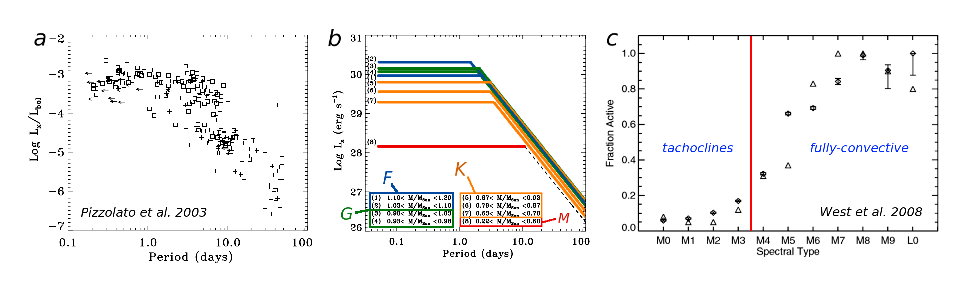
\includegraphics[width=\linewidth]{figs/chapter_1/observational_evidence_pizzolato_2003_west_2008.eps}
  \end{center}
\caption[Observational rotation-activity correlations in main-sequence stars]
	{Observational rotation-activity correlations in main-sequence stars. 
     $(a)$~X-ray activity measured by its luminosity $L_x$ 
          as a function of rotation period, showing
	  growth and saturation phases of the relationship across broad
	  populations of stars.  
     $(b)$~Different stellar types (approximately indicated) saturate
	  at various levels of activity $L_x$ and reach saturation at
	  rotation rates dependent on spectral type.  The growth of
	  activity with more rapid rotation is similar in all G-, K-
	  and M-type stars \citep[adapted from][]{Pizzolato_et_al_2003}.  
     $(c)$~Despite their lack of tachoclines, most fully-convective
  	  stars (types M3.5-M9) show signs of magnetic activity, here
	  measured by H$\alpha$ emission.  
	  Indeed, the fraction of active stars increases with
	  decreasing mass \citep[adapted from][]{West_et_al_2008}.
        \label{fig:observations of stars}}
	\vskip-0.5cm
\end{figure}

Global-scale magnetic activity has also been observed in the
lower-mass main-sequence (dwarf) K- and M-type stars.  
Their convection zones occupy an increasingly large fraction of the interior
and their tachoclines must play a diminishing role in the overall
dynamics, being located in ever deeper regions of the star.  
Even fully convective stars, such as M-dwarfs with masses below
0.35 solar masses, show strong surface magnetism through observations
of H$\alpha$ emission \citep[e.g.,][]{Hawley_et_al_1996, Mohanty&Basri_2003,
West_et_al_2004,West_et_al_2006,West_et_al_2008} and magnetically
sensitive FeH line ratios \citep{Reiners&Basri_2007,
  Reiners&Basri_2008}.  Though these stars
possess no tachoclines and should have distinctly different stellar
dynamos than the sun, there is no observed break in magnetic activity
with stellar type.  Indeed, the fraction of magnetically active stars
increases as the stellar mass decreases (Fig.~\ref{fig:observations of stars}$c$).
These stars also show rotation-activity correlations.  

Recent observations of magnetic fields in a fully convective M-dwarf by
\cite{Donati_et_al_2006} are raising further questions for stellar dynamo
theory.  There, Zeeman Doppler imaging is used to map the surface of the rapidly rotating
and fully convective star v374~Peg.  These observations indicate
strong, organized axisymmetric fields that have strengths of a few
kilo-Gauss but no surface differential rotation.  The global-scale fields appear to be stable
on one-year timescales \citep{Morin_et_al_2008}.  The stable axisymmetric
nature of these fields is in striking contrast to theoretical
predictions for fully convective stars 
\citep[e.g.,][]{Kuker&Rudiger_1999,Kuker&Rudiger_2005_AN, Chabrier&Kuker_2006}. 
Observations of stellar magnetism are indirectly raising 
serious questions about the current paradigm of solar dynamo theory,
where the tachocline is thought to play a crucial role in amplifying and
organizing the global-scale fields and the radial velocity shear of
differential rotation %between the convection zone and interior 
is a necessary ingredient for dynamo action.   

The rotation-activity relationship is tightened across the full range
of solar-like stars when stellar rotation is
given in terms of the Rossby number $\mathrm{Ro} \sim P/\tau_c$, with $P$ the
rotation period and $\tau_c$ an estimate of the convective overturning time
\citep[e.g.,][]{Noyes_et_al_1984a}.  Expressed in this fashion, a common
rotation-activity correlation appears to span spectral types ranging from
late F to late M \citep[e.g.,][]{Patten&Simon_1996, Mohanty&Basri_2003,
  Pizzolato_et_al_2003, Reiners&Basri_2007}. 
These stellar magnetic fields must be generated by dynamo action in
the stellar convection zones.  At present, the rotational dependence
of this dynamo action is unknown.
In mean-field theory, both generation terms are sensitive to rotation
-- the $\alpha$-effect because 
it is proportional to the kinetic helicity of the convective flows, which
sense the overall rotation rate, and the $\Omega$-effect because
more rapidly rotating stars are generally expected to have stronger
differential rotation.  But the detailed nature of these effects in
the solar dynamo and the appropriate scaling with rotation has been
very difficult to elucidate. 


%%% HERE at 4am, 7/30/09

Rotation and stellar magnetism are inextricably linked, as the
stronger magnetic fields in rapidly rotating stars are thought to
produce a larger outward transport of angular momentum by the
magnetized stellar winds, which slowly spin down the stars.    
%Magnetic fields can likewise feed back upon stellar rotation by modifying
%the rate at which angular momentum is lost through a stellar wind
\citep[e.g.,][]{Weber&Davis_1967, Skumanich_1972,
  MacGregor&Brenner_1991, Matt&Pudritz_2008}.
The time needed for significant spindown appears to be a
strong function of stellar mass \citep[e.g.,][]{Barnes_2003, West_et_al_2004}.
Solar-mass stars slow less rapidly than somewhat less massive G and K-type
stars, but still appear to lose much of their angular momentum by the
age of the Hyades (about 1~Gyr).  They spin more slowly yet when 
they are as old as the Sun.  Present day observations of the solar wind
likewise indicate that the current angular momentum flux from the Sun is a few
times 10$^{30}$ dyne~cm \citep[e.g.,][]{Pizzo_et_al_1983}, suggesting a time-scale
for substantial angular momentum loss of a few billion years.   Analyses of stellar spindown
as a function of age and mass have thus provided further constraints on
stellar magnetism and its connections to rotation.   


In addition, recent observations of solar-type stars suggest
that the topology of the global-scale fields changes with rotation rate,
with the rapid rotators having substantial global-scale toroidal
magnetic fields at their surfaces \citep{Petit_et_al_2008}.
The overall picture that emerges from these observations is that rapid
rotation, as realized in the younger Sun and in a host of other stars, can
aid in the generation of strong magnetic fields, and that
young stars tend to be rapidly rotating
and magnetically active, whereas older ones are slower and less active 
\citep[e.g.,][]{Barnes_2003, West_et_al_2004, West_et_al_2008}.  

A full theoretical understanding of the rotation-activity relationship, and
likewise of stellar spindown, has remained elusive.  Some aspects of these
phenomena probably depend upon the details of magnetic flux emergence,
chromospheric and coronal heating, and mass loss mechanisms -- but the
basic existence of a rotation-activity relationship is widely
thought to reflect some underlying rotational dependence of the dynamo
process itself \citep[e.g.,][]{Knobloch_et_al_1981, Noyes_et_al_1984a,
Baliunas_et_al_1996}.

\clearpage
Research into the stellar magnetism of solar-like stars is timely. 
These lower-mass stars are the primary targets of the NASA Kepler
mission and the ESA CoRoT satellite, which both seek to find the
signatures of Earth-like planets orbiting other stars and to perform
asteroseismology on some of these stars.  These
solar-like stars have large habitable zones and are
the closest analogues to our own Sun and solar system.  In the search for their
possible life-bearing worlds, we will learn much more about their host
stars.  Kepler will observe about $10^5$ stars over the course of
the mission, searching for other Earths by the transit method. While
searching for the slight dips in stellar light from these eclipses, the
satellite will make detailed measurements of surface magnetic
activity and differential rotation through high-precision photometry.
For several hundred low-mass stars, Kepler will also carry out
asteroseismology, which will yield new insights into the masses,
sizes and ages of these stars, possibly along with measurements of
their convection zone depths and internal rotation.  Such observations
are likely to lead to a renaissance in stellar physics, challenging our views on
stellar structure, aging processes and stellar magnetism.  A much better understanding
of stellar magnetism and activity may well shed new light on the solar
dynamo and may be crucial for reliably detecting distant Earths.


Probing the nature of these dynamos and the impact of faster rotation on the internal stellar
dynamics requires both accurate observations and detailed dynamical models of
the stellar interiors.  The faster flows of differential rotation are
much easier to detect than the relatively slow motions associated with
meridional circulations; observations across the HR diagram
indicate that differential rotation is a common feature in many stars.
Asteroseismic observations with the Kepler and CoRoT missions may soon begin to
constrain the internal rotation structure.  At present only
measurements of surface differential rotation are available, as assessed
with a variety of techniques including photometric
variability \citep{Donahue_et_al_1996, Walker_et_al_2007}, Doppler
imaging \citep{Donati_et_al_2003} and Fourier transform methods
\citep{Reiners&Schmitt_2003}. 


At our current state of knowledge, stellar magnetism raises three fundamental
questions, which missions like Kepler and CoRoT will begin to address in great
observational detail
\begin{enumerate}
 \item      Where are global-scale magnetic fields built
           and organized within the interiors of stars like our sun?

 \item      Why is there a correlation between rotation rate and magnetic
           activity, and why is this behavior similar in stars with very
	   different convection zone depths?

 \item      What role do tachoclines play in stellar dynamos?
\end{enumerate}
To probe these questions more deeply, we can now turn to simulations
of magnetohydrodynamic (MHD) convection and dynamo action.  These large
computations must be carried out on supercomputers, and these 
theoretical tools are helping to sort out the mysteries of stellar
magnetism. 



\section{Global Models of Stellar Dynamos}
Advances in supercomputing have enabled three-dimensional (3-D)
simulations that are beginning to capture many of
the dynamical elements of the solar convection zone.  Early
global-scale simulations of solar convection by
\citet{Gilman_1975,Gilman_1977,Gilman_1979} under the Boussinesq
approximation were extended by the pioneering work of
\citet{Gilman&Glatzmaier_1981}.  Such global-scale simulations of solar 
convection conducted in full spherical shells sought to capture the largest
scales of convective flows and began to study how they can establish
differential rotation and meridional circulations.  However, the range of
spatial and temporal scales present in solar convection are vast and
thus the computational resources required by the modeling are daunting.

Through recent advances in massively parallel computer architectures,
3-D solar convection simulations are now beginning to make detailed contact with the
observational constraints provided by helioseismology \citep[e.g.,][]{
Brun&Toomre_2002, Miesch_et_al_2006, Miesch_et_al_2008}. Other efforts have focused on
the vigorous turbulence and the dynamo action achieved in the bulk of the 
solar convection zone \citep{Brun_et_al_2004}, with recent studies
beginning to include the tachocline as a region of penetrative
overshoot, shear, and magnetic field amplification \citep{Browning_et_al_2006}.  
Facilitated by these computational advances, models of convection and
dynamo action within the cores of A-type stars have also begun to be
investigated \citep{Browning_et_al_2004, Brun_et_al_2005,
  Featherstone_et_al_2007, Featherstone_et_al_2009}, as have models of fully-convective
M-dwarf stars \citep{Browning_2008} and red giant branch stars
\citep{Palacios&Brun_2007, Brun&Palacios_2009}.

To date, most models of stellar differential rotation and dynamo
action in stars like our Sun that rotate more rapidly have been
carried out in 2-D under the simplifying assumptions of mean-field
theory \citep[e.g.,][]{Rudiger_et_al_1998, Kuker&Stix_2001,
Kuker&Rudiger_2005_A&A, Kuker&Rudiger_2005_AN}.  The 
time is ripe to pursue the question with fully 3-D simulations of
global-scale stellar convection.


%\clearpage
\begin{figure}[!t]
  \begin{center}
    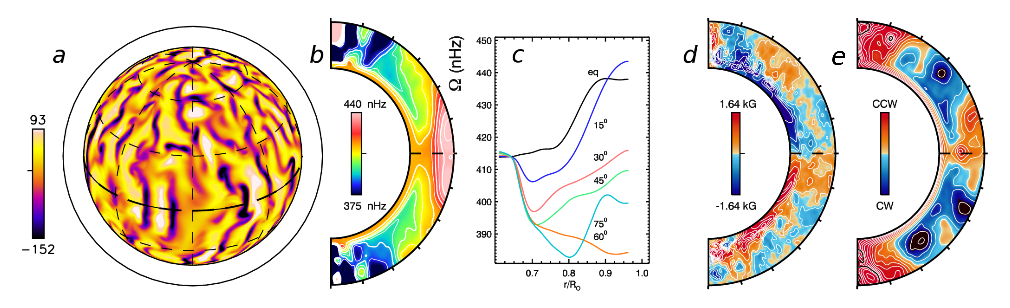
\includegraphics[width=\linewidth]{figs/chapter_1/matt_pen6_Vr_DR_Bphi_Bp.eps}
  \end{center}
    \caption[Snapshot of 3-D ASH solar dynamo simulation which includes a tachocline]
            {Snapshot of 3-D ASH solar dynamo simulation which
              includes a tachocline.  This layer of shear and
              penetration is located at the base  of the convection zone. 
      $(a)$~Radial velocity in orthographic
      projection at $0.88\:R_\sol$, showing the north pole and equatorial
      regions with upflows in light tones and downflows in dark tones (scale in m/s).
      $(b)$~Its mean profile of angular velocity
      $\Omega(r,\theta)$, with a solar-like differential rotation profile
      in the bulk of the convection zone and near uniform rotation in the
      deeper interior. $(c)$~Radial cuts of $\Omega$ at selected
      latitudes.  These simulations are beginning to capture in a
      self-consistent fashion the key ingredients of latitudinal and radial
      shear.
      $(d)$~Profile of temporally- and azimuthally-averaged longitudinal
      magnetic field $\langle B_\phi \rangle$,  
      with substantial mean field present in the
      tachocline and little in the convection zone above.
      $(e)$~Accompanying mean poloidal field lines, with polarity
      indicated by color.  These snapshots are from a model based on
      the simulation of \cite{Browning_et_al_2006}.
      \label{fig:Browning et al tachocline}}
\end{figure}

Simulations of the global-scale solar dynamo have generally affirmed
the view that the tachocline may play a central role in building the
globally-ordered magnetism in the Sun.  Early 3-D
simulations of solar convection without a tachocline
at the base of the convection zone achieved dynamo action and produced
magnetic fields which were strongly dominated by fluctuating
components with little global-scale order \citep{Brun_et_al_2004}.
When a tachocline of penetration and shear was included, remarkable
global-scale structures were realized in the tachocline region, while
the convection zone remained dominated by fluctuating fields
\citep{Browning_et_al_2006}.  These results are illustrated in
Figure~\ref{fig:Browning et al tachocline}.  


These simulations are making good progress 
toward clarifying the elements at work in the operation of the solar
global-scale dynamo, but for
other stars many questions remain.  In particular, observations of
large-scale magnetism in fully convective M-stars 
\citep{Donati_et_al_2006}, along with the persistence of a rotation-activity
correlation in such low-mass stars, hint that perhaps 
tachoclines may not be essential for the generation of global-scale
magnetic fields.  This view is partly borne out by 3-D simulations of
M-dwarfs under strong rotational constraints \citep{Browning_2008}, where
strong longitudinal mean fields were realized despite the
lack of either substantial differential rotation or a stable interior
and thus no classical tachocline.  Major puzzles remain in the quest
to understand stellar magnetism and its scaling with stellar rotation.

With growing computational resources available, the time has come to
extend these solar simulations to broader classes of stars.  
Such studies will enhance our understanding
of stellar dynamo action, by making detailed contact with the evolving
observations of stellar magnetism in stars like our sun.  Studying
dynamo action in other stars is likely to shine new light on the uncertain
physical processes at work within the solar dynamo.  

\section{Convection and Dynamo Action in Rapidly Rotating Suns}
Encouraged by the success of the solar simulations, we have begun
exploring convection and dynamo action in younger and more rapidly
rotating suns in this thesis.   We have found that
younger suns likely possess a much stronger differential rotation
and that the flows of meridional circulation become weaker with more
rapid rotation.  At high rotation rates, the convection becomes strongly
modulated in strength with longitude.  Striking localized patterns
of convection emerge at the equator, and these active nests of
convection dominate the transport of heat and angular momentum in that
region.  At the highest rotation rates, the convection can be entirely
confined to narrow intervals (or active nests) in longitude.  

Modulated convection has persisted under more turbulent conditions and
the active nests of convection appear in some dynamo simulations as well.
When present, these nests of localized convection persist for long intervals of time
and despite their small filling factor maintain a strong differential rotation.
The emergence of spatially localized convective states has been observed in other systems, 
particularly in theoretical studies of doubly-diffusive systems such as thermosolutal convection 
\citep[e.g.,][]{Spina_et_al_1998, Batiste_et_al_2006}, in laboratory studies of convection 
in binary fluids \citep[e.g.,][]{Surko_et_al_1991}, and in simulations of magnetoconvection
where isolated ``convectons'' have been observed \citep{Blanchflower_1999}.  
In shells of rapidly rotating fluid, temporally intermittent patches of localized
convection emerged in Boussinesq simulations of the geodynamo
\citep{Grote&Busse_2000} and in anelastic simulations of convection in
young suns with much deeper convection zones \citep{Ballot_et_al_2006,
Ballot_et_al_2007}.  
In many of these systems, spatial modulation occurs in the weakly nonlinear regime
close to the onset of convection.  In contrast, our simulations
of stellar convection in younger suns are in a regime of fully developed turbulent
convection.

\clearpage
We have begun preliminary simulations of
the dynamo action possible in these stars and have found several
surprises.  These MHD simulations span the
convection zone alone, as the nature of tachoclines in more rapidly
rotating suns is at present unclear.  We find that a variety of
dynamos can be excited, including steady and oscillating states, and
that dynamo action is substantially easier to achieve at these faster
rotation rates than in the solar simulations.  Some of the oscillating
simulations undergo quasi-regular global-scale polarity reversals,
with the mean toroidal and poloidal fields exchanging polarities.  

In these rapidly rotating solar-type stars,
substantial global-scale organization of magnetic
fields can occur in the middle of the convection zone.  These wreaths
of magnetism fill the convection zone and appear to be a general
feature of our dynamos, appearing now in our solar dynamos as well. 
Generally, we find that the dynamos operating in the rapidly rotating
suns may not require the presence of a tachocline, being able to
instead organize global-scale fields in the bulk of their convection zones.



We describe briefly in Chapter~\ref{chapter:ASH} the 3-D
magnetohydrodynamic anelastic spherical harmonic simulation code
called ASH and the parameter space explored by our simulations that
are carried out in spherical shells. In
Chapter~\ref{chapter:convection in G1-G10}, we discuss the nature of
convection realized in more rapidly rotating stars and the emergence
of spatially-localized patterns of convection.  Here we also examine
the global-scale flows realized in our simulations, including
differential rotation and meridional circulation, and their scaling
with more rapid rotation.  A more detailed exploration of the active
nests of convection is presented in Chapter~\ref{chapter:active nests
of convection}.

We then turn to dynamo simulations, examining in
Chapter~\ref{chapter:case D3} the persistent wreaths of magnetism
achieved in a rapidly rotating dynamo rotating at three times the
current solar rate.  In Chapter~\ref{chapter:case D5} we examine
time-dependent behavior and organized global-scale polarity
reversals in a dynamo rotating five times faster than the Sun. 
We return in Chapter~\ref{chapter:dynamo production} to the three solar dynamo 
with persistent magnetic wreaths and examine how those global-scale
structures are created and maintained.   
In Chapter~\ref{chapter:menagerie of dynamos} we explore the broad
parameter space sampled by rapidly rotating dynamos spinning at up to
fifteen times the solar rate.  We find that magnetic wreaths are a
nearly ubiquitous feature in all of these simulations.  Here we also return to the
Sun itself and find wreaths of magnetism as well.  We further briefly consider
convective and dynamo processes at work in older, more slowly spinning
suns. In Chapter~\ref{chapter:the promise of the future} we show
preliminary results for wreath-building dynamos that include
tachoclines of shear and penetration.  We find that magnetic wreaths
continue to fill the convection zone and undergo cycles of polarity
reversal.  Here we summarize our explorations of rapidly rotating
dynamos and look to projects of the future. 

% DONE.  11:30am 7/30/09  Time to tune it.



